\section{Appendix} \label{appendix}


\subsection{NewYorker Data for evaluation}

\begin{figure}[!ht]
\small
\centering
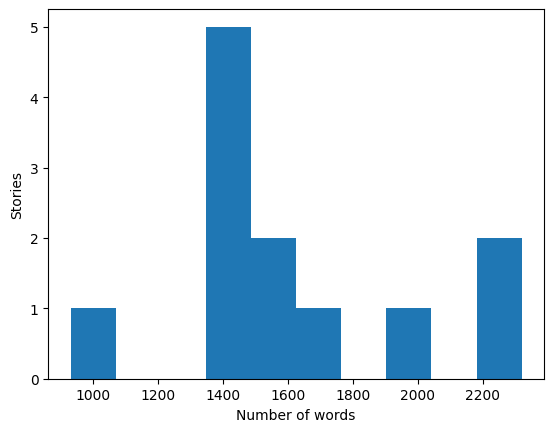
\includegraphics[width=0.4\textwidth]{figures/length.png}
\caption{\label{lengthdist} Distribution of word count of stories in our test set}
\end{figure}

Table \ref{teststories} shows the data used for conducting our evaluation. The 12 stories shown are taken from The New Yorker and summarized into single-sentence plots. These stories come from highly established literary experts acting as an upper bound for what it means to be creative. These stories span complex themes.

\begin{table*}[!ht]
\centering
\small
\def\arraystretch{1.35}
\begin{tabular}{|l|}
\hline
\begin{tabular}[c]{@{}l@{}}Write a New Yorker-style story given the plot below. Make sure it is atleast \textbf{\color{blue}\{\{word\_count\}\}} words. Directly start with the\\ story, do not say things like `Here's the story {[}...{]}:\end{tabular}                                                                                                                                                                                            \\ \hline\hline
\begin{tabular}[c]{@{}l@{}}You wrote the story I gave you below. I requested a story with \textbf{\color{blue}\{\{word\_count\}\}} words, but the story only has\\ \textbf{\color{blue}\{\{current\_word\_count\}\}} words. Can you rewrite the story to make it longer, and closer to the \textbf{\color{blue}\{\{word\_count\}\}} word target\\ I gave you. Directly start with the story, do not say things like `Here's the story {[}...{]}:`\\ \\ Current story: \{\{story\}\}\end{tabular} \\ \hline
\end{tabular}
\vspace{2ex}
\caption{\label{promptstory}Prompt to write the initial story (Row1) vs Prompt to rewrite the initial story to be longer. word\_count represents the number of words in the human written story on a given plot (P) while current\_word\_count represents the number of words in the LLM generated story on the same plot (P)}
\end{table*}

\begin{table*}[!ht]
\def\arraystretch{1.15}
\small
\begin{tabular}{|l|l|}
\hline
Story                                    & Plot                                                                                                                                                                                                                                                                                                                                                                                                                                                                                                                                   \\ \hline
\href{https://www.newyorker.com/books/flash-fiction/a-triangle}{A Triangle}                               & \begin{tabular}[c]{@{}l@{}}An observer becomes entranced by a seemingly ordinary couple on the street, follows them home, and then \\watches them from outside in the rising floodwaters, drawing an eerie connection between the woman and\\ a discarded, burned chair they'd noticed earlier.\end{tabular}                                                                                                                                                                    \\ \hline\hline
\href{https://www.newyorker.com/books/flash-fiction/barbara-detroit-1966}{\begin{tabular}[c]{@{}l@{}}Barbara\\ Detroit,1966\end{tabular}}                    & \begin{tabular}[c]{@{}l@{}}On Feb 12, 1966, a heavily pregnant woman named Barbara experienced a shocking incident in her synagogue\\in Southfield, Detroit, where a young man shot and killed the renowned Rabbi Adler before turning the gun\\ on himself, and though Barbara tried to reach the shooter, she was swept away by the fleeing crowd.\end{tabular}                                                                              \\ \hline\hline
\href{https://www.newyorker.com/books/flash-fiction/beyond-nature}{Beyond Nature}                           & \begin{tabular}[c]{@{}l@{}}A solitary man walking in a remote mountainous region comes across a car crash, and stays by the side\\ of the lifeless female victim, narrating stories of his past and reflecting on the impermanence of \\events and life itself, while awaiting emergency services amidst the looming presence of wilderness.\end{tabular}                                                                                                                \\ \hline\hline
\href{https://www.newyorker.com/books/flash-fiction/certain-european-movies}{\begin{tabular}[c]{@{}l@{}}Certain European\\ Movies\end{tabular}}                  & \begin{tabular}[c]{@{}l@{}}Two individuals, at a residency together, navigate the complexity of their ephemeral relationship during\\ their final beach trip, framed by misadventures, subtle tensions, unspoken desires, and looming departures.\end{tabular}                                                                                                                                                                                   \\ \hline\hline
\href{https://www.newyorker.com/books/flash-fiction/keys}{Keys}                                     & \begin{tabular}[c]{@{}l@{}}Daniel, struggling with recurring dreams of his ex-wife Rachel and a mysterious unused flat, eventually \\discusses them with his current partner Isabel, sparking various reflections and conversations about their\\ past relationships, until a real-life discovery of old keys triggers a nostalgic memory and helps him find a\\ way to reconnect with his present relationship through canoeing.\end{tabular}                                     \\ \hline\hline
\href{https://www.newyorker.com/books/flash-fiction/listening-for-the-click}{\begin{tabular}[c]{@{}l@{}}Listening For\\ the Click\end{tabular}}                  & \begin{tabular}[c]{@{}l@{}}Navigating a complex social landscape, the protagonist experiences a series of complex relationships \\and emotional turmoil in a student environment, and engages in self-discovery and self-reflection as she\\ interacts with the characters Carl, Martin, Lizzy, and Johan, resulting in a journey of introspection,\\ betrayal, love, and personal growth.\end{tabular}                                                          \\ \hline\hline
\href{https://www.newyorker.com/magazine/2023/05/15/maintenance-hvidovre-fiction-olga-ravn}{\begin{tabular}[c]{@{}l@{}}Maintenance,\\ Hvidovre\end{tabular}}                   & \begin{tabular}[c]{@{}l@{}}A woman experiences a disorienting night in a maternity ward where she encounters other similarly \\disoriented new mothers, leading to an uncanny mix-up where she leaves the hospital with a baby \\that she realizes is not her own, yet accepts the situation with an inexplicable sense of happiness.\end{tabular}                                                                                                  \\ \hline\hline
\href{https://www.newyorker.com/magazine/2022/11/14/returns}{Returns}                                  & \begin{tabular}[c]{@{}l@{}}The narrator visits their elderly mother in her small town, spending a day with her that is filled with \\nostalgia, conversation, and old habits, only to return a month later after her hospitalization due to\\ a sunstroke, finding remnants of their last visit.\end{tabular}                                                                                                                                                                      \\ \hline\hline
\href{https://www.newyorker.com/books/flash-fiction/the-facade-renovation-thats-going-well}{\begin{tabular}[c]{@{}l@{}}The Facade \\Renovation\\ That’s Going Well\end{tabular}} & \begin{tabular}[c]{@{}l@{}}An academic faculty housed in a building with a critical waterproofing layer missing experiences a series\\ of disruptive and problematic construction repairs, causing tension, inconvenience, and health concerns\\ among the tenants, ultimately leading to resignation and endurance in hopes of better future circumstances.\end{tabular}                                                        \\ \hline\hline
\href{https://www.newyorker.com/books/flash-fiction/the-kingdom-that-failed}{\begin{tabular}[c]{@{}l@{}}The Kingdom\\ That Failed\end{tabular}}                  & \begin{tabular}[c]{@{}l@{}}The narrator recounts their college friendship with the seemingly flawless Q, and after a decade apart, \\they accidentally cross paths at a pool, where the narrator anonymously observes Q's failed attempt to \\let down a woman about a work-related issue, demonstrating that Q, too, has his share of difficulties.\end{tabular}                                                                                                \\ \hline\hline
\href{https://www.newyorker.com/magazine/2022/06/13/trash }{Trash}                                    & \begin{tabular}[c]{@{}l@{}}A woman unexpectedly marries the son of a successful, ambitious woman named Miss Emily, finding both \\acceptance and critique from her mother-in-law as she navigates this new relationship and confronts the \\stark contrasts between her former life as a supermarket cashier and her new life as part of a well-off family.\end{tabular}                                                                                                            \\ \hline\hline
\href{https://www.newyorker.com/culture/personal-history/the-last-dance-with-my-dad}{\begin{tabular}[c]{@{}l@{}}The Last Dance\\ with my Dad \end{tabular}}               & \begin{tabular}[c]{@{}l@{}}A young teenager recounts her experiences of fitting into her father's gay lifestyle, highlighted by a\\ seven-day cruise with hundreds of gay men, where she experienced acceptance and connection, had her\\ first genuine interaction with a  boy, and shared a last dance with her terminally ill father.\end{tabular}                                                                                                       \\ \hline
\end{tabular}
\vspace{2ex}
\caption{\label{teststories} Expert-written short stories from the New Yorker along with their human-verified GPT4 generated summary as plots that are included as part of our test data for Creativity Evaluation}
\end{table*}


\subsection{Expert Perception on the TTCW tests}

\begin{figure*}[!ht]
    \centering
     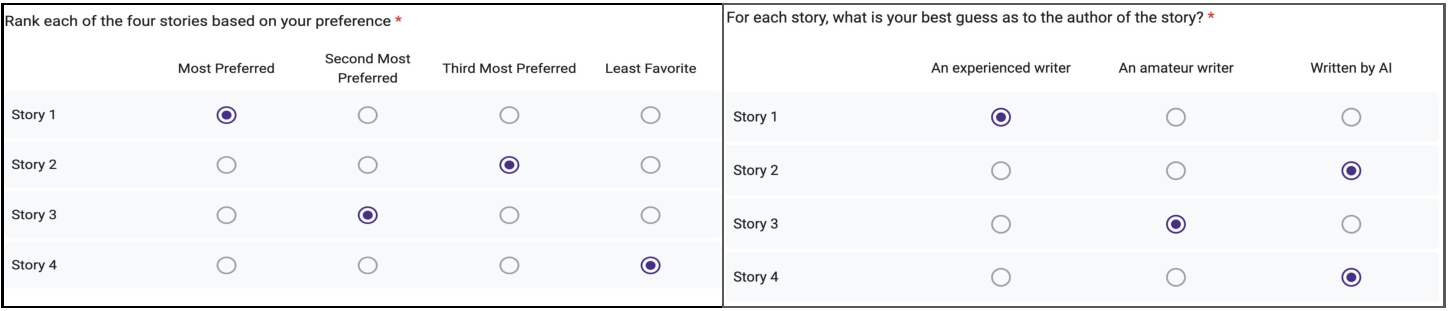
\includegraphics[width=\textwidth]{figures/rel.pdf}
    \caption{\label{relev} Relative Evaluation by Creative Writing Experts within a given group of four stories}
\end{figure*}

\begin{table*}[!ht]
\small
\centering
\begin{tabular}{|l|l|}
\hline
E5 & \begin{tabular}[c]{@{}l@{}}It was a pretty effective rubric! I'm used to being more subjective in my work -- did you like a story? Did it connect with \\you? Did it make sense? Why or why not? It was often challenging to break it down into more regimented segments \\like the rubric asked for -- but I do think that it allowed me to express the subjective feelings in a pretty thorough and\\ structured way!\end{tabular}                                                                                                                                                                 \\ \hline
E3 & \begin{tabular}[c]{@{}l@{}}As for the rubric, I thought it was quite thorough. There were some categories where I would say the story didn’t ``pass,"\\ but which were excellent. This happened often with the categories about multiple points of view, and innovative\\ structure and form. Overall, I think the rubric was helpful in helping me think about the different aspects of storytelling.\end{tabular}                                                                                                                                                                                 \\ \hline
E4 & \begin{tabular}[c]{@{}l@{}}I thought the rubric felt pretty thorough; the only part I felt could be added was that suggestion about consistency in\\ voice \& diction!\end{tabular}                                                                                                                                                         \\ \hline
E2 & \begin{tabular}[c]{@{}l@{}}The rubric seemed great to me! It’s however hard to talk about something like pacing without talking about scene and \\summary, for instance. Or the difference between originality of thought and originality in theme/content—wouldn’t the \\latter make up the former and vice/versa? But it is also comprehensive and I can see the merits of this sort of repetition in\\ teasing out a fuller picture of things\end{tabular} \\ \hline
E1 & \begin{tabular}[c]{@{}l@{}}I thought the rubric was pretty good tbh. I think there is overlap in some of the different elements, like "language \\proficiency \& literary devices" and "originality in thought." it's tricky to use words like "satisfying" and "sophisticated" \\when assessing art, but there's always going to be a great deal of subjectivity in these matters.I think that voice is a crucial \\aspect of high-quality writing that is being overlooked by the rubric, and one that greatly informs how I as a reader\\ evaluate 
and appreciate literary writing.\end{tabular} \\ \hline
\end{tabular}
\vspace{2ex}
\caption{\label{expertfeedbackrubric}Expert perception and feedback on the TTCW tests they conducted as part of our data collection.}
\end{table*}

Since the experts listed in Table \ref{creativeexperts} were not involved in designing the rubric but evaluated several stories based on the rubric we asked them their \textit{overall thought about the rubric and any potentially crucial test we missed out on that they use to discriminate between good and bad writing}.As can be seen in Table \ref{expertfeedbackrubric} in Appendix overall almost every expert agreed on the thorough and effective nature of our rubric. Many of them agreed on the fact that our rubric helped them to think about different aspects of storytelling in a more structured way. One of the difficult things about coming up with a rubric for creativity is ensuring coverage. Even though our rubric covers most aspects of creative writing, some experts such as E1 and E4 emphasized on the utility of \textbf{Consistency of Voice and Diction} as a measurable test. In E4's words \textit{``Inconsistent voice and diction are sometimes/often notable in stories that aren't very good, and when voice \& diction are used beautifully, it enhances a story considerably"}. E1 similarly exclaimed \textit{``One of the most meaningful aspects of high-quality literary writing is voice, which conveys qualities of proficiency, artistry, personality, and identity."}. We hope future work can adapt this as a meaningful test in addition to the tests covered in our rubric. Finally, some of the tests from our rubric can have potential overlaps as pointed out by E2. This is further corroborated by the similar numbers for \textit{Narrative Pacing} and \textit{Scenes vs Exposition} suggesting a strong correlation between the two.
\begin{table*}[!ht]
\small
\centering
% \def\arraystretch{1.3}
\begin{tabular}{|l|l|l|}
\hline
Test & Passing Stories & Failing Stories \\ \hline
\begin{tabular}[c]{@{}l@{}}Originality in\\ Form\end{tabular} & \begin{tabular}[c]{@{}l@{}}Inventive techniques like time jumping, varied \\ perspectives, unconventional punctuation, and\\ delayed revelation of key information\end{tabular} & \begin{tabular}[c]{@{}l@{}}Conventional and linear in its form, language, \\ and narrative, with occasional attempts at \\ innovation that do not significantly contribute to \\ its overall originality or creativity\end{tabular} \\ \hline
\begin{tabular}[c]{@{}l@{}}Originality in\\ Thought\end{tabular} & \begin{tabular}[c]{@{}l@{}}Fresh language, unique plot and characters, subtle\\ emotional resonance, and inventive metaphors. Minor \\ familiar elements, but do not undermine the overall \\ sense of imagination and distinctiveness\end{tabular} & \begin{tabular}[c]{@{}l@{}}Stories relies heavily on cliches \& tired tropes.\\ Language does not feel fresh or original with \\ narrative arc following a predictable trajectory.\\ Metaphors, descriptions, and overall premise \\ cover familiar ground that lacks novelty or nuance\end{tabular} \\ \hline
\begin{tabular}[c]{@{}l@{}}Originality in\\ Theme/Content\end{tabular} & \begin{tabular}[c]{@{}l@{}}Unconventional, dreamlike exploration of emotions\\ such as love and loss, evoking empathy and reflection\\ through its distinct main character perspective, \\ eschewing simplistic meanings for ambiguity, and \\ valuing open-ended questions over singular messages,\\ thus providing a unique reading experience compared\\ to conventional stories.\end{tabular} & \begin{tabular}[c]{@{}l@{}}Disjointed narrative, underdeveloped themes, \\ inconsistent tone, vaguely defined characters, and\\ abrupt context shifts, lack depth and fail to provide \\ substantive insight or originality to the reader.\end{tabular} \\ \hline\hline
\begin{tabular}[c]{@{}l@{}}World Building\\ and Setting\end{tabular} & \begin{tabular}[c]{@{}l@{}}Strategic use of concrete, specific sensory details from\\ a particular character’s perspective balances narrative\\ momentum, making a fictional world feel real, vivid\\ and immersive for readers. Thoughtful depiction of\\ everyday objects, and idiosyncratic elements within\\ narrative and dialogue to balance exposition with \\ vivid scene-setting, creating authenticity and realism \\ that serves the plot and characters\end{tabular} & \begin{tabular}[c]{@{}l@{}}Fictional world is not always convincingly \\established through sensory details and language. \\Stories rely too heavily on overwrought imagery\\ and figurative language without grounding \\the reader in a tangible reality.\end{tabular} \\ \hline
\begin{tabular}[c]{@{}l@{}}Character\\ Development\end{tabular} & \begin{tabular}[c]{@{}l@{}}Fully realized characters with contradictions, \\ motivations, and backstories that make them\\ feel lifelike. Flatter, less developed characters\\ that feel appropriate for the narrative goals \\ and style is not necessarily a weakness\end{tabular} & \begin{tabular}[c]{@{}l@{}}Characters not well rounded. easily resorting to \\stereotypes. Predictable arcs not making them\\memorable. Actions or motivations unclear leading \\to disconnect\end{tabular} \\ \hline
\begin{tabular}[c]{@{}l@{}}Rhetorical\\ Complexity\end{tabular} & \begin{tabular}[c]{@{}l@{}}Rich subtext that emerges through contrasts between\\ characters and settings. Omissions that let readers \\ fill in meaning, metaphors with layered significance, \\ implicit characterization, ambiguous endings, \\ intertextual references, and rich language that goes\\ beyond straightforward storytelling\end{tabular} & \begin{tabular}[c]{@{}l@{}}Straightforward storytelling, lack of complexity,\\ nuance, and ambiguity.The absence of context and \\ ironic tensions, overtelling instead of showing, \\ Use of expository dialogue, blunt symbolism, \\ predictable characters, and definitive endings, all \\of which limit interpretation and undermine\\ their potential resonance\end{tabular} \\ \hline
\end{tabular}
\vspace{2ex}
\caption{\label{expertexpl2}Common themes and issues found in expert explanations for tests focusing on TTCW-Originality and TTCW-Elaboration}
\vspace{-8ex}
\end{table*}

\subsection{Common themes in TTCW of Originality and Elaboration}


Table~\ref{expertexpl2} provides common themes and issues found in the expert explanations for each TTCW in the Originality and Elaboration dimensions.


\subsection{Example LLM-generated and expert-written explanations for a TTCW assessment} 

\begin{table*}[!ht]
\centering
\small
\def\arraystretch{1.35}
\begin{tabular}{|l|l|}
\hline
GPT4 & \begin{tabular}[c]{@{}l@{}}The story incorporates numerous instances of subtext that serve to further develop the characters' internal emotions \\ and relationships, as well as accentuate the atmospheric tension and undertones of longing. The subtext, which is\\ subtly weaved into surface-level interactions, actions, and observations, is eloquently crafted and does not feel \\ forced, enriching both the narrative depth and setting.\\ One key passage with evident subtext is when he is in the ocean, swimming and jumping off the rock, while she\\ observes from the towel. The surface-level interpretation suggests a casual, relaxed beach day. However, the \\ subtext is rife with allusions of emotional undercurrents in their interaction. His unawareness of her going \\ into the water parallels the emotional disconnect between them, insinuating the vast, metaphorical space that \\ separates their respective experiences and understanding of their relationship.\\ Another instance of subtext occurs when he takes a photo of her with her swimsuit top off, indicating his attraction\\ to her. But the meaning deepens when we understand that he will delete the photo before going home, implicitly\\ revealing his guilt or fear of being discovered, and again highlighting the transient, secret nature of their relationship.\\ The line, "As in certain European movies" suggests the fleeting, impermanent element of their relationship and the\\ eventual abruptness and intensity of feelings that often feature in said films. The 'European movies' serve as a \\ metaphor for the unexpected and sudden end of their encounter. \\ In these examples, the subtext does not feel forced but instead flows naturally from the characters and \\ circumstances, subtly conveying deeper meanings that heighten both the narrative tension and emotional depth.\\ \\ So Yes.\end{tabular} \\ \hline
E3   & \begin{tabular}[c]{@{}l@{}}There is rich subtext, as the main character seems continually conflicted about whether she wants to be where she is, \\ doing what she is doing. On the surface, she is carefree, riding to the beach with the guy she met, skipping the ceramics\\ and the museum, and whatever else. And yet, she is unhappy and unsatisfied, longing for a beer, imagining that if their\\ relationship continued they would only hate each other. This tension is maintained throughout the story.\end{tabular}                                                                                                                                                                                                                                                                                                               \\ \hline
E1   & \begin{tabular}[c]{@{}l@{}}This piece has an iceberg of subtext floating underneath it. The entire story is conveyed through the successful \\ integration of subtext and text. The interactions between the protagonist and the man (Did you see me jump of the \\ rock? No, she hadn't.Did he notice she had gone in the water too, that her hair was dripping? No, he hadn't.)convey\\ a profound disconnect that causes the reader to wonder why the protagonist continues to suffer the presence of this\\ man she clearly disdains and seems to view as an incompetent man-child.\end{tabular}
               \\ \hline
E7   & \begin{tabular}[c]{@{}l@{}}Yes!!!!! Again, the idea of the story was fairly simple (the inevitability of age, parting, change), but it was illustrated\\ in a way that felt inspiring re: questioning how these ideas relate and resonate throughout our own lives. It was really \\ beautiful and I was left feeling changed at the end of it :)\end{tabular}                                                                                                                                                                                                                                                            \\ \hline
\end{tabular}
\vspace{2ex}
\caption{\label{llmvsexpertexpl}LLM explanation vs expert explanation for Rhetorical Complexity}
\end{table*}

In Table~\ref{llmvsexpertexpl}, we show examples of explanations that experts wrote in conjunction with a binary TTCW assessment they made on a story, as well as the corresponding LLM-generated explanations.

\subsection{Can non-experts administer TTCW tests?}

Recruiting experts for data annotation purposes is challenging, and costly, and must consider the time constraint put on the experts. Prior work has shown the potential of crowd-sourcing (through platforms such as Amazon Mechanical Turk) and the ability of non-experts to accomplish complex tasks as a crowd \cite{kittur2013future}, when following an appropriate workflow that iterates and validates the work on individual non-experts. Some prior work has even shown the validity of crowd-based feedback for writing tasks \cite{bernstein2010soylent,nebeling2016wearwrite}. 

In this work, we chose to rely on experts for annotation, to maximize the validity of our experiments, and confirm whether experts with domain knowledge would reach satisfying agreement levels when evaluating stories with TTCW. Future work can leverage our open-sourced annotations to explore whether non-experts correlate with experts when performing TTCW evaluation, which could lead to more cost-effective TTCW evaluation.

\subsection{Prompts for TTCW} \label{allprompts}

All the instructions shown to creative writing experts and LLMs are given in the tables below.


\begin{table*}[!ht]
\centering
\small
\begin{tabular}{|l|l|}
\hline
\begin{tabular}[c]{@{}l@{}}Expert \\ Measure\end{tabular}               & Does the manipulation of time in terms of compression or stretching feel appropriate and balanced?                                                                                                                                    \\ \hline
\begin{tabular}[c]{@{}l@{}}Expanded\\ Expert\\ Measure (M)\end{tabular} & \begin{tabular}[c]{@{}l@{}}`Compression/stretching of time' in fiction writing, also known as pacing, refers to the manipulation of time in \\storytelling for dramatic effect, pacing, or other narrative purposes. Essentially, it's about controlling the perceived \\speed and rhythm at which a story unfolds.\\ \\

Compression of time refers to when events that take a long time (hours, days, weeks, or even years) are summarized \\or condensed into a brief narrative span. For example, a writer might compress several years of a character's life \\into a few paragraphs to quickly convey important changes or developments.\\ \\

On the other hand, stretching of time is when a brief moment or event is drawn out over pages or chapters. It's often \\used to create suspense, emphasize details, or delve deeper into a character's thoughts and feelings. For example, \\the few seconds it takes for a dropped glass to hit the floor might be stretched out with detailed descriptions of the\\ action, reactions, and thoughts of characters involved.\\ \\

Storytime refers to the time within the world of the story, while real-world time refers to the time it takes for the \\reader to read the story. A skilled writer can manipulate the relationship between these two to affect the pacing of \\the narrative, either speeding it up (compression) or slowing it down (stretching). This technique plays a crucial role \\in shaping the reader's experience and engagement with the story.\end{tabular} \\ \hline
\begin{tabular}[c]{@{}l@{}}Human\\ Instruction\end{tabular}             & \begin{tabular}[c]{@{}l@{}}\{\{M\}\}\\ \\ Based on the story that you just read, answer the following question.\\ \textit{\color{blue}Does the manipulation of time in terms of compression or stretching feel appropriate and balanced?}\\ -Yes \\ -No \\\\ Reasoning : \end{tabular}                                                                       \\ \hline
\begin{tabular}[c]{@{}l@{}}LLM\\ Instruction\end{tabular}               & \begin{tabular}[c]{@{}l@{}}\{\{M\}\}\\ \\ Given the story above, list out the scenes in the story in which time compression or time stretching is used, and \\argue for each whether it is successfully implemented.  Then overall, give your reasoning about the question below \\and give an answer to it between 'Yes' or 'No' only \\ \\ \textit{\color{blue} Q) Does the manipulation of time in terms of compression or stretching feel appropriate and balanced?}\end{tabular}                                                                                                                                                                                                                    \\ \hline
\end{tabular}
\vspace{2ex}
\caption{\label{prompting}TTCW Fluency1 (Narrative Pacing) }
\vspace{-5ex}
\end{table*}


% ==================================================





\begin{table*}[!ht]
\centering
\small
% \def\arraystretch{1.15}
\begin{tabular}{|l|l|}
\hline
\begin{tabular}[c]{@{}l@{}}Expert \\ Measure\end{tabular}               & \begin{tabular}[c]{@{}l@{}}Does the story have an appropriate balance between scene and summary/exposition or it relies on one\\ of the elements heavily compared to the other?  \end{tabular}                                                                                                                                  \\ \hline
\begin{tabular}[c]{@{}l@{}}Expanded\\ Expert\\ Measure (M)\end{tabular} & \begin{tabular}[c]{@{}l@{}}'Scene' and 'summary/exposition' are two crucial elements of narrative storytelling, and balancing them \\appropriately is an important skill in fiction writing.\\ \\ 

A 'scene' is a moment in the story that is dramatized in real-time. Scenes are usually vivid and engaging, often \\featuring character interaction, dialogue, and action. They are the building blocks of the plot, and through them, \\the story unfolds.\\ \\ 

'Summary' or 'exposition', on the other hand, involves summarizing events or providing information. Instead of \\unfolding in real time, \\summaries compress time and tell the reader what happened. Exposition provides \\necessary background information, like character history, setting details, or prior events. \\ \\ 

A good writer knows when to use scenes to make the story come alive, show character development, or increase \\tension. They also know when to use summary or exposition to move the story forward, fill in background \\information, or bridge gaps between important scenes. \\ \\ 

The right balance between scene and summary/exposition can vary depending on the story, but in general, it's \\essential for maintaining a good pace, keeping the reader engaged, and delivering necessary information. \\A story with too many scenes and not enough summary might feel overwhelming or slow, while a story with \\too much exposition and not enough scenes could feel dry and unengaging.\end{tabular} \\ \hline
\begin{tabular}[c]{@{}l@{}}Human\\ Instruction\end{tabular}             & \begin{tabular}[c]{@{}l@{}}\{\{M\}\}\\ \\ Based on the story that you just read, answer the following question.\\ \textit{\color{blue} Does the story have an appropriate balance between scene and summary/exposition or it relies on one of the elements} \\\textit{\color{blue}heavily compared to the other?} \\ -Yes \\ -No \\\\ Reasoning : \end{tabular}    
\\ \hline
\begin{tabular}[c]{@{}l@{}}LLM\\ Instruction\end{tabular}               & \begin{tabular}[c]{@{}l@{}}\{\{M\}\}\\ \\ Given the story above, answer the following question. Please first explain your reasoning step by step \\and then given an answer between 'Yes' or 'No' only \\ \\ \textit{\color{blue} Does the story have an appropriate balance between scene and summary/exposition or it relies on one of the elements} \\\textit{\color{blue}heavily compared to the other?}\end{tabular}                                                                                                                                                                                                                    \\ \hline
\end{tabular}
\vspace{2ex}
\caption{\label{prompting}TTCW Fluency2 (Scene vs Exposition) }
\vspace{-5ex}
\end{table*}


% ==================================================


\begin{table*}[!ht]
\centering
\small
% \def\arraystretch{1.15}
\begin{tabular}{|l|l|}
\hline
\begin{tabular}[c]{@{}l@{}}Expert \\ Measure\end{tabular}               & Does the story make sophisticated use of idiom or metaphor or literary allusion?                                                                                                                                     \\ \hline
\begin{tabular}[c]{@{}l@{}}Expanded\\ Expert\\ Measure (M)\end{tabular} & \begin{tabular}[c]{@{}l@{}}`Idiom' refers to phrases or expressions that have a figurative, or sometimes literal, meaning that is \\comprehensible to a particular group of people. These can be cultural, regional, or specific to a certain group or \\profession.Sophisticated use of idiom suggests that the writer is skillfully using these expressions to lend \\authenticity to character voices or to convey specific meanings in a concise way.\\\\

`Metaphor' is a figure of speech that describes an object or action in a way that isn't literally true, but helps explain\\ an idea or make a comparison. Sophisticated use of metaphor suggests the
writer could create impactful, original \\comparisons that reveal deeper insights about themes,
characters, or situations in the story.\\\\

`Literary allusion' refers to a brief and indirect reference to a person, place, thing or idea of
historical, cultural,\\ literary, or political significance. It does not describe in detail the person or thing to which it refers. A sophisticated\\ use of literary allusion implies the writer can effectively incorporate these references to enhance the depth\\ and resonance of the story. They can provide contextual richness, evoke a specific tone, or draw parallels between\\ the narrative and the work alluded to.\\\\

Overall, when a writer uses these techniques well, they add depth, interest, and nuanced \\meaning
to their work. It allows for a richer reading experience, where the literal events are \\imbued with deeper symbolic or thematic significance.\end{tabular} \\ \hline
\begin{tabular}[c]{@{}l@{}}Human\\ Instruction\end{tabular}             & \begin{tabular}[c]{@{}l@{}}\{\{M\}\}\\ \\ Based on the story that you just read, answer the following question.\\ \textit{\color{blue}Does the story make sophisticated use of idiom or metaphor or literary allusion?}\\ -Yes \\ -No \\\\ Reasoning: \end{tabular}                                                                       \\ \hline
\begin{tabular}[c]{@{}l@{}}LLM\\ Instruction\end{tabular}               & \begin{tabular}[c]{@{}l@{}}\{\{M\}\}\\ \\ Given the story above, please list out all the metaphors, idioms and literary allusions, and for each decide \\whether it is successful vs it feels forced or too easy.  Then overall, give your reasoning about the question \\below and give an answer to it between 'Yes' or 'No' only\\ \\ \textit{\color{blue} Q) Does the story make sophisticated use of idiom or metaphor or literary allusion?}\end{tabular}                                                                                                                                                                                                                    \\ \hline
\end{tabular}
\vspace{2ex}
\caption{\label{prompting}TTCW Fluency3 (Language Proficiency \& Literary Devices) }
\vspace{-5ex}
\end{table*}


% ==================================================



\begin{table*}[!ht]
\centering
\small
% \def\arraystretch{1.15}
\begin{tabular}{|l|l|}
\hline
\begin{tabular}[c]{@{}l@{}}Expert \\ Measure\end{tabular}               & Does the end of the story feel natural and earned, as opposed to arbitrary or abrupt?                                                                                                                                    \\ \hline
\begin{tabular}[c]{@{}l@{}}Expanded\\ Expert\\ Measure (M)\end{tabular} & \begin{tabular}[c]{@{}l@{}}If the writer ends the piece simply because they are 'tired of writing', the conclusion might feel abrupt, disjointed, \\or unfulfilling to the reader. It suggests a rushed ending, where plot threads might be left unresolved and character \\arcs incomplete.\\ \\ 

Conversely, if the writer concludes because they've reached `the moment the entire piece has been leading readers \\towards', it implies a well-considered and purposeful ending. The events, character development, and themes \\throughout the story have built towards this climactic moment, providing a satisfying resolution to the reader.\\ \\ 

A strong ending offers a sense of closure, ties up the central conflicts or questions of the story, and generally \\leaves the reader feeling that the narrative journey was worthwhile and complete.\end{tabular} \\ \hline
\begin{tabular}[c]{@{}l@{}}Human\\ Instruction\end{tabular}             & \begin{tabular}[c]{@{}l@{}}\{\{M\}\}\\ \\ Based on the story that you just read, answer the following question.\\ \textit{\color{blue}Does the end of the story feel natural and earned, as opposed to arbitrary or abrupt?}\\ -Yes \\ -No \\\\ Reasoning : \end{tabular}                                                                       \\ \hline
\begin{tabular}[c]{@{}l@{}}LLM\\ Instruction\end{tabular}               & \begin{tabular}[c]{@{}l@{}}\{\{M\}\}\\ \\ Given the story above, answer the following question. Please first explain your reasoning step by step \\ and then given an answer between 'Yes' or 'No' only\\ \\ \textit{\color{blue} Q) Does the end of the story feel natural and earned, as opposed to arbitrary or abrupt?}\end{tabular}                                                                                                                                                                                                                    \\ \hline
\end{tabular}
\vspace{2ex}
\caption{\label{prompting}TTCW Fluency4 (Narrative Ending) }
\vspace{-5ex}
\end{table*}



% ==================================================



\begin{table*}[!ht]
\centering
\small
% \def\arraystretch{1.15}
\begin{tabular}{|l|l|}
\hline
\begin{tabular}[c]{@{}l@{}}Expert \\ Measure\end{tabular}               & Do the different elements of the story work together to form a unified, engaging, and satisfying whole?                                                                                                                                     \\ \hline
\begin{tabular}[c]{@{}l@{}}Expanded\\ Expert\\ Measure (M)\end{tabular} & \begin{tabular}[c]{@{}l@{}}A well-crafted story usually follows a logical path, where the events in the beginning set up the middle, which then\\ logically leads to the end. Every scene, character action, and piece of dialogue should serve the story and propel it \\forward. Well-written stories have an underlying the unity that binds the elements together. The themes, plotlines, \\character arcs, and other elements of the story interweave to create a harmonious whole. A story with 'disorder'\\ might feel disjointed, with characters, scenes, etc that don't connect or contribute to the overall narrative.\end{tabular} \\ \hline
\begin{tabular}[c]{@{}l@{}}Human\\ Instruction\end{tabular}             & \begin{tabular}[c]{@{}l@{}}\{\{M\}\}\\ \\ Based on the story that you just read, answer the following question.\\ \textit{\color{blue}Do the different elements of the story work together to form a unified, engaging, and satisfying whole?}\\ -Yes \\ -No \\\\ Reasoning : \end{tabular}                                                                       \\ \hline
\begin{tabular}[c]{@{}l@{}}LLM\\ Instruction\end{tabular}               & \begin{tabular}[c]{@{}l@{}}\{\{M\}\}\\ \\ Given the story above, answer the following question. Please first explain your reasoning step by step and then \\give an answer between 'Yes' or 'No' only\\ \\ \textit{\color{blue} Q) Do the different elements of the story work together to form a unified, engaging, and satisfying whole?}\end{tabular}                                                                                                                                                                                                                                 \\ \hline
\end{tabular}
\vspace{2ex}
\caption{\label{prompting}TTCW Fluency5 (Understandability \& Coherence) }
\vspace{-5ex}
\end{table*}


% ==================================================



\begin{table*}[!ht]
\centering
\small
% \def\arraystretch{1.15}
\begin{tabular}{|l|l|}
\hline
\begin{tabular}[c]{@{}l@{}}Expert \\ Measure\end{tabular}               & \begin{tabular}[c]{@{}l@{}}Does the story provide diverse perspectives, and if there are unlikeable characters, are their perspectives \\presented convincingly and accurately? \end{tabular}                                                                                                                                     \\ \hline
\begin{tabular}[c]{@{}l@{}}Expanded\\ Expert\\ Measure (M)\end{tabular} & \begin{tabular}[c]{@{}l@{}}A good writer can convincingly and accurately depict a wide range of character viewpoints, including those of\\ characters who may be morally ambiguous, difficult, or otherwise unappealing.\\ \\ 

This can involve diving into the mindset of characters who may act or think in ways that the reader, or even \\the writer, finds objectionable or repugnant. It involves understanding their motivations, their beliefs, and the \\reasons behind their actions, and then conveying these elements in a way that is believable and consistent.\\ \\ 

The purpose of doing so is not to justify or endorse these perspectives, but rather to create complex, three-\\dimensional characters who contribute to the richness and depth of the story. This can also serve to \\challenge the reader, provoke thought, and provide insights into different aspects of the human experience.\end{tabular} \\ \hline
\begin{tabular}[c]{@{}l@{}}Human\\ Instruction\end{tabular}             & \begin{tabular}[c]{@{}l@{}}\{\{M\}\}\\ \\ Based on the story that you just read, answer the following question.\\ \textit{\color{blue}Does the story provide diverse perspectives, and if there are unlikeable characters, are their perspectives presented} \\ \textit{\color{blue}convincingly and accurately?}\\ -Yes \\ -No \\\\ Reasoning : \end{tabular}                                                                       \\ \hline
\begin{tabular}[c]{@{}l@{}}LLM\\ Instruction\end{tabular}               & \begin{tabular}[c]{@{}l@{}}\{\{M\}\}\\ \\ Given the story above, answer the following question. Please first explain your reasoning step by step and then \\give an answer between 'Yes' or 'No' only\\ \\ \textit{\color{blue} Q) Does the story provide diverse perspectives, and if there are unlikeable characters, are their perspectives presented}\\\textit{\color{blue} convincingly and accurately?}\end{tabular}                                                                                                                                                                                                                                 \\ \hline
\end{tabular}
\vspace{2ex}
\caption{\label{prompting}TTCW Flexibility1 (Perspective \& Voice Flexibility) }
\vspace{-5ex}
\end{table*}


% ==================================================




\begin{table*}[!ht]
\centering
\small
% \def\arraystretch{1.15}
\begin{tabular}{|l|l|}
\hline
\begin{tabular}[c]{@{}l@{}}Expert \\ Measure\end{tabular}               & \begin{tabular}[c]{@{}l@{}}Does the story achieve a good balance between interiority and exteriority, in a way that feels \\emotionally flexible? \end{tabular}                                                                                                                                     \\ \hline
\begin{tabular}[c]{@{}l@{}}Expanded\\ Expert\\ Measure (M)\end{tabular} & \begin{tabular}[c]{@{}l@{}}`Emotional flexibility' is asking whether the piece of writing effectively balances action and introspection, and \\if it portrays a broad and realistic spectrum of emotions.\\ \\

`Exteriority' refers to the observable actions, behaviors, or dialogue of a character, and the physical or visible \\aspects of the setting, plot, and conflicts.\\ \\

`Interiority', on the other hand, pertains to the inner life of a character — their thoughts, feelings, memories, \\and subjective experiences.\\ \\

A balance between these two aspects is crucial in creating well-rounded characters and compelling narratives. \\If a piece is too heavy on exteriority, it may feel shallow or lack emotional depth. If it leans too much on\\ interiority, it could become overly introspective and potentially lose the momentum of the plot.
\end{tabular} \\ \hline
\begin{tabular}[c]{@{}l@{}}Human\\ Instruction\end{tabular}             & \begin{tabular}[c]{@{}l@{}}\{\{M\}\}\\ \\ Based on the story that you just read, answer the following question.\\ \textit{\color{blue}Does the story achieve a good balance between interiority and exteriority, in a way that feels emotionally flexible?}\\ -Yes \\ -No \\\\ Reasoning : \end{tabular}                                                                       \\ \hline
\begin{tabular}[c]{@{}l@{}}LLM\\ Instruction\end{tabular}               & \begin{tabular}[c]{@{}l@{}}\{\{M\}\}\\ \\ Given the story above, answer the following question. Please first explain your reasoning step by step and \\then give an answer between 'Yes' or 'No' only\\ \\ \textit{\color{blue}Q) Does the story achieve a good balance between interiority and exteriority, in a way that feels} \\\textit{\color{blue}emotionally flexible?}\end{tabular}                                                                                                                                                                                                                                 \\ \hline
\end{tabular}
\vspace{2ex}
\caption{\label{prompting}TTCW Flexibility2 (Emotional Flexibility) }
\vspace{-5ex}
\end{table*}


% ==================================================




\begin{table*}[!ht]
\centering
\small
% \def\arraystretch{1.15}
\begin{tabular}{|l|l|}
\hline
\begin{tabular}[c]{@{}l@{}}Expert \\ Measure\end{tabular}               & \begin{tabular}[c]{@{}l@{}}Does the story contain turns that are both surprising and appropriate? \end{tabular}                                                                                                                                     \\ \hline
\begin{tabular}[c]{@{}l@{}}Expanded\\ Expert\\ Measure (M)\end{tabular} & \begin{tabular}[c]{@{}l@{}}`Surprising': This refers to the element of unpredictability in a narrative. A good story often has plot twists, \\character developments, or thematic revelations that surprise the reader, subverting their expectations in a \\thrilling way.It's about keeping readers engaged and curious, never fully knowing what's going to happen next.\\ \\ 

`Appropriate': Despite the surprises and twists, the turns in the story must also make sense within the established \\context of the story's universe, its characters, and its themes. This means that even though an event might be \\surprising, it should feel appropriate or fitting in hindsight. It shouldn't feel like the writer has broken the rules \\they've set up, or made a character behave inconsistently without reason, simply for the sake of shock value.\\ \\ 

So when someone wonders if a writer can make turns that are 'both surprising and appropriate', they're asking \\if the writer can strike this balance between unexpectedness and coherence, keeping the reader on their toes \\while maintaining a believable, satisfying narrative. \end{tabular} \\ \hline
\begin{tabular}[c]{@{}l@{}}Human\\ Instruction\end{tabular}             & \begin{tabular}[c]{@{}l@{}}\{\{M\}\}\\ \\ Based on the story that you just read, answer the following question.\\ \textit{\color{blue}Does the story contain turns that are both surprising and appropriate?}\\ -Yes \\ -No \\\\ Reasoning: \end{tabular}                                                                       \\ \hline
\begin{tabular}[c]{@{}l@{}}LLM\\ Instruction\end{tabular}               & \begin{tabular}[c]{@{}l@{}}\{\{M\}\}\\ \\ Given the story above, list each element in the story that is intended to be surprising. For each, decide whether the\\ surprising element remains appropriate with respect to the entire story. Then overall, give your reasoning \\about the question below and give an answer to it between 'Yes' or 'No' only\\ \\ \textit{\color{blue} Q) Does the story contain turns that are both surprising and appropriate?}\end{tabular}                                                                                                                                                                                                                                 \\ \hline
\end{tabular}
\vspace{2ex}
\caption{\label{prompting}TTCW Flexibility3 (Structural Flexibility) }
\vspace{-5ex}
\end{table*}


% ==================================================






\begin{table*}[!ht]
\centering
\small
% \def\arraystretch{1.15}
\begin{tabular}{|l|l|}
\hline
\begin{tabular}[c]{@{}l@{}}Expert \\ Measure\end{tabular}               & \begin{tabular}[c]{@{}l@{}}Will an average reader of this story obtain a unique and original idea from reading it? \end{tabular}                                                                                                                                     \\ \hline
\begin{tabular}[c]{@{}l@{}}Expanded\\ Expert\\ Measure (M)\end{tabular} & \begin{tabular}[c]{@{}l@{}}If a story is good, the reader gains new insights, perspectives, or knowledge from it. This doesn't necessarily\\ mean factual information but could relate to a deeper understanding of human nature, cultural insights,\\ unique viewpoints, or even the exploration of new ideas and themes. Essentially, it's about what\\ the reader takes away from the story beyond just the plot.\\ \\ 

A good story has lasting impacts on its readers and the society. It is meant to entertain, inform, provoke \\thought, challenge beliefs, provide comfort, or raise awareness on specific issues.
 \end{tabular} \\ \hline
\begin{tabular}[c]{@{}l@{}}Human\\ Instruction\end{tabular}             & \begin{tabular}[c]{@{}l@{}}\{\{M\}\}\\ \\ Based on the story that you just read, answer the following question.\\ \textit{\color{blue}Will an average reader of this story obtain a unique and original idea from reading it?}\\ -Yes \\ -No \\\\ Reasoning : \end{tabular}                                                                       \\ \hline
\begin{tabular}[c]{@{}l@{}}LLM\\ Instruction\end{tabular}               & \begin{tabular}[c]{@{}l@{}}\{\{M\}\}\\ \\ Given the story above, list out elements that are unique takeaways of this story for the reader. Then overall, \\give your reasoning about the question below and give an answer to it between 'Yes' or 'No' only\\ \\ \textit{\color{blue} Q) Will an average reader of this story obtain a unique and original idea from reading it?}\end{tabular}                                                                                                                                                                                                                                 \\ \hline
\end{tabular}
\vspace{2ex}
\caption{\label{prompting}TTCW Originality1 (Originality in Theme and Content) }
\vspace{-3ex}
\end{table*}


% ==================================================








\begin{table*}[!ht]
\centering
\small
% \def\arraystretch{1.15}
\begin{tabular}{|l|l|}
\hline
\begin{tabular}[c]{@{}l@{}}Expert \\ Measure\end{tabular}               & \begin{tabular}[c]{@{}l@{}}Is the story an original piece of writing without any cliches?\end{tabular}                                                                                                                                     \\ \hline
\begin{tabular}[c]{@{}l@{}}Expanded\\ Expert\\ Measure (M)\end{tabular} & \begin{tabular}[c]{@{}l@{}}A cliche is an idea, expression, character, or plot that has been overused to the point of losing its original \\meaning or impact. They often become predictable and uninteresting for the reader. Originality suggests\\ that the piece isn't cliche.

 \end{tabular} \\ \hline
\begin{tabular}[c]{@{}l@{}}Human\\ Instruction\end{tabular}             & \begin{tabular}[c]{@{}l@{}}\{\{M\}\}\\ \\ Based on the story that you just read, answer the following question.\\ \textit{\color{blue}Is the story an original piece of writing without any cliches?}\\ -Yes \\ -No \\\\ Reasoning: \end{tabular}                                                                       \\ \hline
\begin{tabular}[c]{@{}l@{}}LLM\\ Instruction\end{tabular}               & \begin{tabular}[c]{@{}l@{}}\{\{M\}\}\\ \\ Given the story above, are there any cliches in the story? If so, list out all the elements in this story that \\are cliche. Then overall, give your reasoning if the piece is negatively impacted by the cliches and give \\an answer to the question below between 'Yes' or 'No' only\\ \\ \textit{\color{blue} Q) Is the story an original piece of writing without any cliches?}\end{tabular}                                                                                                                                                                                                                                 \\ \hline
\end{tabular}
\vspace{2ex}
\caption{\label{prompting}TTCW Originality2 (Originality in Thought) }
\vspace{-5ex}
\end{table*}


% ==================================================




\begin{table*}[!ht]
\centering
\small
% \def\arraystretch{1.15}
\begin{tabular}{|l|l|}
\hline
\begin{tabular}[c]{@{}l@{}}Expert \\ Measure\end{tabular}               & \begin{tabular}[c]{@{}l@{}}Does the story show originality in its form?\end{tabular}                                                                                                                                     \\ \hline
\begin{tabular}[c]{@{}l@{}}Expanded\\ Expert\\ Measure (M)\end{tabular} & \begin{tabular}[c]{@{}l@{}}When someone says that a piece of fiction 'shows an innovative use of form/structure', they're referring to\\ how the writer has chosen to shape and organize the story in an unusual, original, or inventive way. This could \\involve a variety of different elements, including:\\ \\ 

Narrative Structure: This could include unconventional timelines (e.g. a non-linear story, a story told in reverse)\\, multiple perspectives or narrators, or unusual narrative voices (e.g. a story told from the perspective of an \\inanimate object).\\ \\ 

Format: This could be something as simple as using unconventional punctuation or capitalization, or as complex \\as telling a story through a series of letters, diary entries, newspaper clippings, or other documents. In recent years,\\ some authors have even experimented with using social media posts or text messages as a form of narrative structure.\\ \\ 

Genre Hybridity: Combining elements from different genres or sub-genres in unexpected ways can also be seen\\ as an innovative use of form such as Horror-Mystery or Comic Fantasy.\\ \\ 

Plot Structure: Deviating from traditional plot structures such as three-act structure, or following them in unexpected\\ ways.For example, telling a story without a clear resolution, incorporating multiple climaxes or using revelation as a \\device where a surprising, and often shocking, development occurs that was previously kept hidden from the \\characters and/or the audience. It's typically designed to provide new context for interpreting what has previously \\occurred in the story. \\ \\ 

Language and Style: Innovative use of form can also come in the form of unique use of language, style, or \\even typography, such as concrete poetry or writing that visually represents its subject matter on the page.\\ \\ 

The goal of this innovation is often to provide a fresh reader experience, challenge conventional reading\\ expectations, or to create a deeper or more complex exploration of the story's themes.

 \end{tabular} \\ \hline
\begin{tabular}[c]{@{}l@{}}Human\\ Instruction\end{tabular}             & \begin{tabular}[c]{@{}l@{}}\{\{M\}\}\\ \\ Based on the story that you just read, answer the following question.\\ \textit{\color{blue}Does the story show originality in its form?}\\ -Yes \\ -No \\\\ Reasoning: \end{tabular}                                                                       \\ \hline
\begin{tabular}[c]{@{}l@{}}LLM\\ Instruction\end{tabular}               & \begin{tabular}[c]{@{}l@{}}\{\{M\}\}\\ \\ Given the story and the devices mentioned above, list each device used with a short explanation of whether it is \\successful or not. Then overall, give your reasoning about the question below and give an answer to it\\ between 'Yes' or 'No' only\\ \\ \textit{\color{blue} Q) Does the story show originality in its form?}\end{tabular}                                                                                                                                                                                                                                 \\ \hline
\end{tabular}
\vspace{2ex}
\caption{\label{prompting}TTCW Originality3 (Originality in Form) }
\vspace{-5ex}
\end{table*}


% ==================================================




\begin{table*}[!ht]
\centering
\small
% \def\arraystretch{1.15}
\begin{tabular}{|l|l|}
\hline
\begin{tabular}[c]{@{}l@{}}Expert \\ Measure\end{tabular}               & \begin{tabular}[c]{@{}l@{}}Does each character in the story feel developed at the appropriate complexity level, ensuring that no character \\feels like they are present simply to satisfy a plot requirement?\end{tabular}                                                                                                                                     \\ \hline
\begin{tabular}[c]{@{}l@{}}Expanded\\ Expert\\ Measure (M)\end{tabular} & \begin{tabular}[c]{@{}l@{}} A `flat character' is typically a minor character who is not thoroughly developed or who does not undergo \\significant change or growth throughout the story. They often embody or represent a single trait or idea, \\and they're used to advance the plot or highlight certain qualities in other characters.\\ \\ 

A `complex character', also known as a round character, has depth in feelings and passions, has a variety \\of traits of a real human being, and evolves over time. They have their strengths, weaknesses, \\and they learn from their experiences. They tend to be more engaging to the reader, as they mirror \\the complexity of real people.\\ \\ 

In good stories, authors take a character who initially appears to be one-dimensional or stereotypical (flat) and \\add depth to them. This could be done by revealing more about their backstory, introducing unexpected traits \\or motivations, or having them grow and change in response to the events of the story. \\This transformation from a flat to a complex character can make the narrative more engaging and believable.
 \end{tabular} \\ \hline
\begin{tabular}[c]{@{}l@{}}Human\\ Instruction\end{tabular}             & \begin{tabular}[c]{@{}l@{}}\{\{M\}\}\\ \\ Based on the story that you just read, answer the following question.\\  \textit{\color{blue} Q) Does each character in the story feel developed at the appropriate complexity level, ensuring that no character} \\ \textit{\color{blue}feels like they are present simply to satisfy a plot requirement?}\\ -Yes \\ -No \\\\ Reasoning: \end{tabular}                                                                       \\ \hline
\begin{tabular}[c]{@{}l@{}}LLM\\ Instruction\end{tabular}               & \begin{tabular}[c]{@{}l@{}}\{\{M\}\}\\ \\ Given the story above, list each character and the level of development. Then overall, give your reasoning \\about the question below and give an answer to it between 'Yes' or 'No' only\\ \\ 
 \textit{\color{blue} Q) Does each character in the story feel developed at the appropriate complexity level, ensuring that no character} \\ \textit{\color{blue}feels like they are present simply to satisfy a plot requirement?}\end{tabular}                                                                                                                                                                                                                                 \\ \hline
\end{tabular}
\vspace{2ex}
\caption{\label{prompting}TTCW Elaboration2 (Character Development) }
\vspace{-5ex}
\end{table*}


% ==================================================



\begin{table*}[!ht]
\centering
\small
% \def\arraystretch{1.15}
\begin{tabular}{|l|l|}
\hline
\begin{tabular}[c]{@{}l@{}}Expert \\ Measure\end{tabular}               & \begin{tabular}[c]{@{}l@{}}Are there passages in the story that involve subtext and when there is subtext, does it enrich the story's setting \\or does it feel forced?\end{tabular}                                                                                                                                     \\ \hline
\begin{tabular}[c]{@{}l@{}}Expanded\\ Expert\\ Measure (M)\end{tabular} & \begin{tabular}[c]{@{}l@{}} `Surface' level: This is the most apparent and straightforward level of a story. It includes the visible actions, \\explicit dialogue, and clear descriptions. This is what literally happens in the plot: the characters' actions, events, \\and the apparent consequences.\\ \\ 

`Subtext' level: This is the underlying or implicit meaning that isn't directly stated but can be inferred from \\the characters'  actions, dialogue, and other elements of the story. Subtext often reveals deeper truths about \\characters, themes, or the overall message of the piece. It could be a hidden motive, an unstated\\ emotion, a cultural commentary, or a symbolic meaning.\\ \\ 

For example, in a conversation between two characters, the surface text might be polite and cordial, but the \\subtext \\discerned from the characters' nonverbal cues, previous interactions, or the context of their conversation\\ — could suggest tension or hostility.\\ \\ 

Effective fiction often operates on both levels. The surface text keeps the reader engaged with the plot and \\characters, while the subtext provides depth, complexity, and additional layers of interpretation, \\contributing to a richer and more rewarding reading experience.
 \end{tabular} \\ \hline
\begin{tabular}[c]{@{}l@{}}Human\\ Instruction\end{tabular}             & \begin{tabular}[c]{@{}l@{}}\{\{M\}\}\\ \\ Based on the story that you just read, answer the following question.\\  \textit{\color{blue} Q) Are there passages in the story that involve subtext and when there is subtext, does it enrich the story's setting} \\ \textit{\color{blue} or does it feel forced?}\\ -Yes \\ -No \\\\ Reasoning: \end{tabular}                                                                       \\ \hline
\begin{tabular}[c]{@{}l@{}}LLM\\ Instruction\end{tabular}               & \begin{tabular}[c]{@{}l@{}}\{\{M\}\}\\ \\ Given the story above, answer the following question. Please first explain your reasoning step by step \\and then give an answer between 'Yes' or 'No' only\\ \\ 
 \textit{\color{blue} Q)Are there passages in the story that involve subtext and when there is subtext, does it enrich the story's setting} \\ \textit{\color{blue} or does it feel forced?}\end{tabular}                                                                                                                                                                                                                                 \\ \hline
\end{tabular}
\vspace{2ex}
\caption{\label{prompting}TTCW Elaboration3 (Rhetorical Complexity) }
\vspace{-5ex}
\end{table*}


% ==================================================
